\documentclass[../open-optimization/open-optimization.tex]{subfiles}

\begin{document}


\section{Knapsack Problem}
Knapsack problem can take different forms depending on if the variables are binary or integer.  The binary version means that there is only one item of each item type that can be taken.
\begin{general}{Binary Knapsack Problem}{\npcomplete}
Given an non-negative weight vector $a \in \Q^n_+$, a capacity $b \in \Q_+$, and objective coefficients $c \in \Q^n$, 
\begin{equation}
\begin{split}
\max \ \ & c^\top x\\
\text{s.t.}\ \ & a^\top x \leq b\\
& x \in \{0,1\}^n
\end{split}
\end{equation}
\end{general}
\begin{figure}[H]
\begin{center}
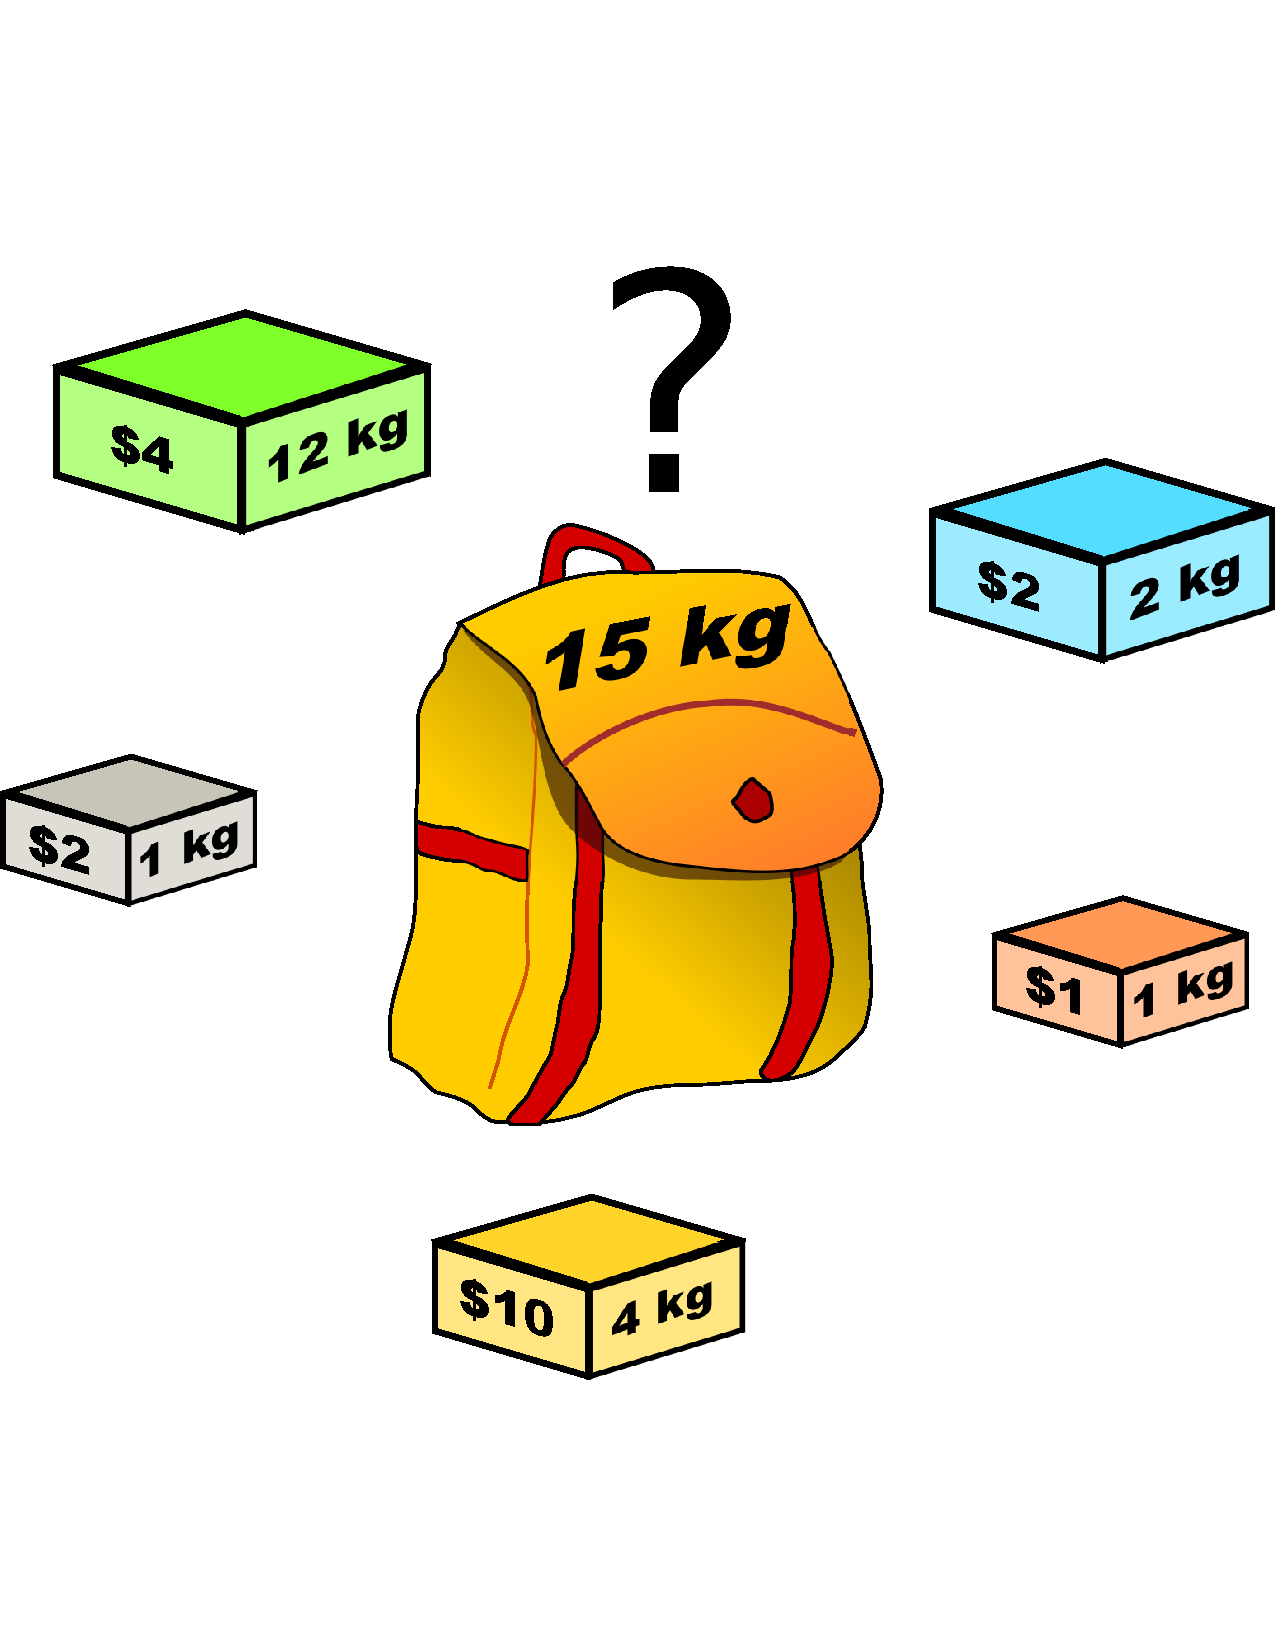
\includegraphics[scale = 0.2]{knapsack}\footnotemark \end{center}
\label{fig:knapsack}
\caption{Knapsack Problem: which items should we choose take in the knapsack that maximizes the value while respecting the 15kg weight limit?}
\end{figure}
\footnotetext{\url{https://en.wikipedia.org/wiki/Knapsack_problem}}

\begin{examplewithcode}{Knapsack}{code:knapsack}
\label{example:knapsack}
You have a knapsack (bag) that can only hold W = 15 kgs.  There are 5 items that you could possibly put into your knapsack.  The items (weight, value) are given as:
(12 kg, $\$$4), (2 kg, $\$$2), (1kg, $\$$2), (1kg, $\$$1), (4kg, $\$$10).  Which items should you take to maximize your value in the knapsack?\\

\noindent \textbf{Variables:}
\begin{itemize}
\item let $x_i = 0$ if item $i$ is in the bag
\item let $x_i = 1$ if item $i$ is not in the bag
\end{itemize}
\textbf{Model:}
\begin{equation}
\begin{split}
\max  \  \ &4 x_1 + 2 x_2 + 2 x_3 + 1 x_4 + 10 x_5\\
\text{ s.t. }\ \ &  12 x_1 + 2 x_2 + 1 x_3 + 1 x_4 + 4 x_5 \leq 15\\
& x_i \in \{0,1\} \text{ for } i=1, \dots, 5
\end{split}
\end{equation}
\end{examplewithcode}
In the integer case, we typically require the variables to be non-negative integers, hence we use the notation $x \in \Z^n_+$.  This setting reflects the fact that instead of single individual items, you have item types of which you can take as many of each type as you like that meets the constraint.
\begin{general}{Integer Knapsack Problem}{\npcomplete}
Given an non-negative weight vector $a \in \Q^n_+$, a capacity $b \in \Q_+$, and objective coefficients $c \in \Q^n$, 
\begin{equation}
\begin{split}
\max \ \ & c^\top x\\
\text{s.t.}\ \ & a^\top x \leq b\\
& x \in \Z^n_+
\end{split}
\end{equation}
\end{general}
We can also consider an equality constrained version
\begin{general}{Equality Constrained Integer Knapsack Problem}{\nphard}
Given an non-negative weight vector $a \in \Q^n_+$, a capacity $b \in \Q_+$, and objective coefficients $c \in \Q^n$, 
\begin{align}
\max \ \ & c^\top x\\
\text{s.t.}\ \ & a^\top x = b\\
& x \in \Z^n_+
\end{align}
\end{general}
\begin{example}
\label{ex:min-coins}
Using pennies, nickels, dimes, and quarters, how can you minimize the number of coins you need to to make up a sum of $83\cent$? 

\textbf{Variables:}
\begin{itemize}
\item Let $p$ be the number of pennies used
\item Let $n$ be the number of nickels used
\item Let $d$ be the number of dimes used
\item Let $q$ be the number of quarters used
\end{itemize}
\textbf{Model}
\begin{align*}
\min \quad & p + n + d + q & \text{ total number of coins used}\\
\text{ s.t. } \quad & p + 5n + 10d + 25 q = 83 & \text{sums to } 83 \cent\\
& p,d,n,q \in \Z_+ & \text{each is a non-negative integer}
\end{align*}
\end{example}
\section{Set Covering}
\begin{general}{Set Covering}{\npcomplete}
\label{general:set-covering}
Given a set $V$ with subsets $V_1, \dots, V_l$, determine the smallest subset $S \subseteq V$ such that 
$S \cap V_i \neq \emptyset$ for all $i=1, \dots, l$.

The set cover problem can be modeled as
\begin{equation}
\begin{split}
\min \ \ & \one^\top x\\
\text{s.t.} \ \ & \sum_{v \in V_i} x_v \geq 1 \text{ for all } i =1, \dots, l \\ 
& x_v \in \{0,1\} \text{ for all } v \in V
\end{split}
\end{equation}
where $x_v$ is a 0/1 variable that takes the value $1$ if we include item $j$ in set $S$ and $0$ if we do not include it in the set $S$.  
\end{general}
\begin{general}{Vertex Cover}{\npcomplete}
Given a graph $G = (V,E)$ of vertices and edges, we want to find a smallest size subset $S \subseteq V$ such that every for every $e = (v,u) \in E$, either $u$ or $v$ is in $S$.   

We can write this as a mathematical program in the form:
\begin{equation}
\begin{split}
\min \ \ & \one^\top x\\
\text{s.t.} \ \ & x_u + x_v \geq 1 \text{ for all } (u,v) \in E \\ 
& x_v \in \{0,1\} \text{ for all } v \in V.
\end{split}
\end{equation}
\end{general}
\begin{examplewithcode}{Vertex Cover}{code:vertex-cover}
\label{example:vertex-cover}
Consider the graph with nodes
\begin{equation}
V = \text{["You", "Ginger", "Juan", "Jameis", "Bob", "Geoff", "Jane"]}
\end{equation}
and edges
\begin{align}E = \text{[["You", "Ginger"],
     ["You", "Juan"], 
     ["You", "Jameis"],
     ["You", "Bob"],}\\
     \text{["You", "Jane"],
     ["You", "Geoff"],
     ["Ginger", "Jameis"],
     ["Jameis", "Bob"],}\\
     \text{
     ["Bob", "Jane"],
     ["Bob", "Geoff"],
     ["Geoff", "Jane"]]}
  \end{align}
%  \includegraphics{}
  
This problem can be modeled as
\begin{alignat*}{1}\min\quad & x_{\text{You}} + x_{\text{Ginger}} + x_{\text{Juan}} + x_{\text{Jameis}} + x_{\text{Bob}} + x_{\text{Geoff}} + x_{\text{Jane}}\\
\text{Subject to} \quad & x_{\text{You}} + x_{\text{Ginger}} \geq 1\\
 & x_{\text{You}} + x_{\text{Juan}} \geq 1\\
 & x_{\text{You}} + x_{\text{Jameis}} \geq 1\\
 & x_{\text{You}} + x_{\text{Bob}} \geq 1\\
 & x_{\text{You}} + x_{\text{Jane}} \geq 1\\
 & x_{\text{You}} + x_{\text{Geoff}} \geq 1\\
 & x_{\text{Ginger}} + x_{\text{Jameis}} \geq 1\\
 & x_{\text{Jameis}} + x_{\text{Bob}} \geq 1\\
 & x_{\text{Bob}} + x_{\text{Jane}} \geq 1\\
 & x_{\text{Bob}} + x_{\text{Geoff}} \geq 1\\
 & x_{\text{Geoff}} + x_{\text{Jane}} \geq 1\\
 & x_{i} \in \{0,1\} \quad\forall i \in \{\text{You,Ginger,\dots,Geoff,Jane}\}\\
\end{alignat*}
\end{examplewithcode}

\begin{examplewithcode}{Southwestern Airways\footnotemark}{code:southwestern-airways}
\label{example:southwestern-airways}
Southwestern Airways needs to assign its crews to cover all its upcoming flights.  We will focus on the problem of assigning three crews based in San Francisco to the flights listed in the first column of the below table.  The other 12 columns show feasible sequences of flights for a crew.  (The numbers in each column indicate the order of the flights: 1 = first stop, 2 = second stop, 3 = third stop...etc.) Exactly three of the sequences need to be chosen (one per crew) in such a way that every flight is covered. (It is permissible to have more than one crew on a flight, where extra crews would fly as passengers, but union contracts require that the extra crews would still need to be paid for their time as if they were working.) The cost of assigning a crew to a particular sequence of flights is given (in thousands of dollars) in the bottom row of the table.  The objective is to minimize the total cost of the three crew assignments that cover all the flights.

\includegraphics[scale = 0.2]{flightcrew.jpg}\footnotemark

\paragraph{Sets}
Let $I = \{1,\dots, 12\}$ denote flight sequences
Let $F = \{1, \dots, 11\}$ denote the flights.
For each flight $i$, let $F_i \subseteq I$ be the set of flight sequences that intersects flight $i$.
\paragraph{Variables}
Let $x_i = 1$ if flight sequence $i$ is chosen and $0$ otherwise
\paragraph{Model}
The model is to minimize cost while respecting that flights are covered.  This can be modeled as 
\begin{align*}
\min \ \ & c^\top x\\
\text{s.t.} \ \ &  \sum_{j \in F_i} x_j \geq 1 & \text{ for all } i=1, \dots, 11\\
& x_j \in \{0,1\}  & \text{ for all } j=1, \dots, 12
\end{align*}

Plugging in the data creates the following integer program:
\begin{align*}\min\quad & 2 x_{1} + 3 x_{2} + 4 x_{3} + 6 x_{4} + 7 x_{5} + 5 x_{6} + 7 x_{7} + 8 x_{8} + 9 x_{9} + 9 x_{10} + 8 x_{11} + 9 x_{12}\\
\text{Subject to} \quad & x_{1} + x_{4} + x_{7} + x_{10} \geq 1\\
 & x_{2} + x_{5} + x_{8} + x_{11} \geq 1\\
 & x_{3} + x_{6} + x_{9} + x_{12} \geq 1\\
 & x_{4} + x_{7} + x_{9} + x_{10} + x_{12} \geq 1\\
 & x_{1} + x_{6} + x_{10} + x_{11} \geq 1\\
 & x_{4} + x_{5} + x_{9} \geq 1\\
 & x_{7} + x_{8} + x_{10} + x_{11} + x_{12} \geq 1\\
 & x_{2} + x_{4} + x_{5} + x_{9} \geq 1\\
 & x_{5} + x_{8} + x_{11} \geq 1\\
 & x_{3} + x_{7} + x_{8} + x_{12} \geq 1\\
 & x_{6} + x_{9} + x_{10} + x_{11} + x_{12} \geq 1\\
 & x_{1} + x_{2} + x_{3} + x_{4} + x_{5} + x_{6} + x_{7} + x_{8} + x_{9} + x_{10} + x_{11} + x_{12} = 3\\
 & x_{i} \in \{0,1\} \quad\forall i \in \{1,2,\dots,11,12\}\\
\end{align*}

\end{examplewithcode}
\footnotetext{This example was taken from Hillier and Lieberman}
\footnotetext{This image table was taken from Hillier and Lieberman}

\begin{general}{Set Covering - Matrix description}{\npcomplete}
\label{general:set-covering-alternate}
Given a non-negative matrix $A \in \{0,1\}^{m \times n}$, a non-negative vector, and an objective vector $c \in \R^n$, the set cover problem is
\begin{equation}
\begin{split}
\max \ \ & c^\top x\\
\text{s.t.}. \ \ & Ax \geq \one \\
& x \in \{0,1\}^n.
\end{split}
\end{equation}
\end{general}
\begin{examplewithcode}{Vertex Cover with matrix}{code:vertex-cover-matrix}
An alternate way to solve \nameref{example:vertex-cover} is to define the adjacency matrix $A$ of the graph.  The adjacency matrix is a $|E| \times |V|$ matrix with $\{0,1\}$ entries.  The each row corresponds to an edge $e$ and each column corresponds to a node $v$.  For an edge $e = (u,v)$, the corresponding row has a $1$ in columns corresponding to the nodes $u$ and $v$, and a 0 everywhere else.  Hence, there are exactly two 1's per row.  Applying the formulation above in \nameref{general:set-covering-alternate} solves the problem.
\end{examplewithcode}


\subsubsection{General Set Covering}
We could also allow for a more general type of set covering where we have non-negative integer variables and a right hand side that has values other than $1$.
\begin{general}{Set Covering - Generalized}{\npcomplete}
\label{general:set-covering-alternate}
Given a non-negative matrix $A \in \Z_+^{m \times n}$, a non-negative vector $b \in \Z^m$, and an objective vector $c \in \R^n$, the set cover problem is
\begin{equation}
\begin{split}
\max \ \ & c^\top x\\
\text{s.t.}. \ \ & Ax \geq b \\
& x \in\Z^n_+.
\end{split}
\end{equation}
\end{general}

\begin{example}{Nurse Scheduling}{--- Adapted from "Applied Integer Programming". exercise 2.6 and 2.7}
\end{example}
Nurses in large hospitals usually work 3 days a week. Daily demand for nurses is summarized in Table 2.4. Determine the number of nurses required per schedule type so that the total wage cost is minimized.
\begin{enumerate}
\item  Use the numbers (not symbols) in the table to model this problem instance.
\item Solve this instance and submit the code.
\item Let $S$ denote the set of schedule types.  How many variables of each type (continuous, binary, integer) does your model have in terms of the number of schedules $|S|$?
\item If part-time nurses are hired at the rate of $\$175$/day, formulate the problem to minimize the total cost. 
\item If part-time nurses must be accompanied by at least three full-time nurses, how would you formulate this constraint?
\end{enumerate}
\begin{table}[h]
\begin{center}
\begin{tabular}{l|ccccc|c}
\hline
\hline
& & & Schedule Type & & \\
\hline
Day & 1 & 2 & 3 & 4 & 5 & Nurses Required\\
\hline
Monday & X & & X & & & 20\\
Tuesday & X & &  &  & X & 25\\
Wednesday & & & X & X & & 26\\
Thursday& & X & & & X& 26\\
Friday & & X & & X & X & 30\\
Saturday& & X& & X& & 30\\
Sunday& X& & X & && 35\\
\hline
Weekly wage& 525 & 470 & 550 & 500 & 425\\
\hline 
\hline
\end{tabular}
\end{center}
\end{table}

\begin{itemize}
		\item Let 
		$$
		x_i = \textrm{The number of nurses to assign to schedule } i\ \forall\ i \in \left\lbrace 1,2,...,5 \right\rbrace.
		$$
\end{itemize}	
		\vspace{.25in}
		The model is
		\begin{align*}
		\textrm{Minimize}	\hspace{.25in}	525x_1+470x_2+550x_3+500x_4+425x_5&&&&
		\end{align*}
		\vspace{-.43in}
		\begin{align*}
		\textrm{s.t.} 		\hspace{.6in}	x_1+x_3 &\geq 20							\\
											x_1+x_5 &\geq 25							\\
											x_3+x_4 &\geq 26							\\
											x_2+x_5 &\geq 26							\\
										x_2+x_4+x_5 &\geq 30							\\
											x_2+x_4 &\geq 30							\\
											x_1+x_3 &\geq 35							\\
												x_i &\in \mathbb{Z}_+ & &\forall\ i \in \left\lbrace 1,2,...,5 \right\rbrace
		\end{align*}
		
		The table tells us which schedule types contribute to each day's staff; i.e. Mondays are staffed entirely by nurses assigned to schedule types 1 and 3, Tuesdays by those assigned to type 1 and 5, and so on. At least 20 nurses are required to be on duty on Mondays; so the number of nurses assigned to schedules 1 and 3 should be at least 20. That is,
			$$
			x_1+x_3 \geq 20.
			$$
		Extending this logic to each day gives us all seven constraints. \\
		
		Alternately, by replacing the X's in the table with 1's we are left with a constraint matrix $S$. Let $\vec{x}^\top = [x_1,x_2,x_3,x_4,x_5]$ be the decision variables and $\vec{r}^\top=[20,25,26,26,30,30,35]$ describe the nurses required for each day, so that
			$$
			S\ \vec{x} \geq \vec{r}
			$$
		describes all seven constraints. 
		%This is the approach taken in the sample code below.

\section{Machine Assignment}


Example Model: Machine assignment\\

\begin{minipage}{0.6\textwidth}
\begin{itemize}
	\item Given $m$ machines and $n$ jobs, find a least cost assignment
	of jobs to machines not exceeding the machine capacities.
	\item Each job $j$ requires $a_{ij}$ units of machine $i$'s capacity $b_i$.
	\item Cost of assigning job $j$ to machine $i$ is $c_{ij}$.
	\end{itemize}
\end{minipage}
\begin{minipage}{0.3\textwidth}
\includegraphics[scale = 0.5]{assignment}
\end{minipage}


Here is a model....  \textbf{To be added....}

\section{Facility Location}
\url{https://en.wikipedia.org/wiki/Facility_location_problem}

\includegraphics[scale = 0.5]{facility-location}

\subsection{Capacitated Facility Location}
\begin{equation}
\begin{array}{rl}
\min & \displaystyle\sum_{i=1}^n\sum_{j=1}^mc_{ij}y_{ij}+\sum_{i=1}^nf_ix_i \\
\text{s.t.} & \displaystyle\sum_{i=1}^ny_{ij}=1 \text{ for all }j=1,\dots,m \\
& \displaystyle \sum_{j=1}^md_jy_{ij}\leqslant u_ix_i\text{ for all }i=1\dots,n \\
&y_{ij}\geqslant0\text{ for all }i=1,\dots,n \text{ and }j=1,\dots,m\\
&x_i\in\{0,1\}\text{ for all } i=1,\dots,n
\end{array}
\end{equation}

\subsection{Uncapacitated Facility Location}
\begin{equation}
\begin{array}{rl}
\min & \displaystyle\sum_{i=1}^n\sum_{j=1}^mc_{ij}z_{ij}+\sum_{i=1}^nf_ix_i \\
\text{s.t.} & \displaystyle\sum_{i=1}^nz_{ij}=1 \text{ for all }j=1,\dots,m \\
& \displaystyle \sum_{j=1}^mz_{ij}\leqslant Mx_i\text{ for all }i=1\dots,n \\
&z_{ij}\in\{0,1\}\text{ for all }i=1,\dots,n \text{ and }j=1,\dots,m\\
&x_i\in\{0,1\}\text{ for all } i=1,\dots,n
\end{array}
\end{equation}


\section{Capital Budgeting}
	\textcolor{blue}{A firm has $n$ projects it could undertake to maximize revenue, but budget limitations require that not all can be completed.}\\
	\textcolor{blue}{Project $j$ expects to produce revenue $c_j$\\
		Project $j$ requires investment $a_{ij}$ in time period $i$ for $i = 1,\ldots,m$\\
		In time period $i$, capital $b_i$ is available}
		
		Let $x_i$ be a binary variable such that $x_i = 1$ if we choose investment $i$ and $x_i = 0$ otherwise.  The the model can be given as:
	\begin{align*}
	\max ~~~& \sum_{j = 1}^n c_jx_j\\
	s.t. ~~~&\sum_{j = 1}^n a_{ij}x_j\leq b_i, ~~~i = 1,\ldots m\\
	& x_j \in \{0,1\} , \ j = 1,\ldots,n
	\end{align*}


Consider the example given in the following table.
	\begin{table}[h]
		\centering
		\resizebox{\columnwidth}{!}{%
			\begin{tabular}{|c|c|c|c|}%[<+->]
				\hline
				Project & $\mathbb{E}$[Revenue] & Resources required in week 1 & Resources required in week 2\\\hline
				\rowcolor{bluegreen} 1 & 10 & 3 & 4\\
				\hline
				2 & 8 & 1 & 2\\\hline
				\rowcolor{bluegreen} 3 & 6 & 2 & 1\\
				\hline
				Resources available & & 5 & 6\\
				\hline
		\end{tabular}}
	\end{table}
	$$
	\max~~~~~ 10x_1+8x_2+6x_3
	$$
	subject to
	\begin{align*}
	3x_1+1x_2+2x_3\leq5\\
	4x_1+2x_2+1x_3\leq6\\
	x_j \in \{0,1\},\  j = 1,2,3
	\end{align*}



\section{Network Flow}

\section{Transportation Problem}
\url{https://www.youtube.com/watch?v=Jr7LI-sUEmo}
\subsection{Modeling Tricks}
In this section, we describe ways to model a variety of constraints that commonly appear in practice.  The goal is changing constraints described in words to constraints defined by math.
\subsection{Either Or Constraints}
\emph{``At least one of these constraints holds"} is what we would like to model.  Equivalently, we can phrase this as an \emph{inclusive or} constraint.  
\begin{general}{Either Or}{}{}

\begin{equation}
\text{Either} \ \ \ a^\top x \leq b\ \  \text{  or  } \ \  c^\top x \leq d \ \ \text{holds} 
\end{equation}
can be modeled as 
\begin{equation}
\begin{split}
a^\top x - b &\leq M_1 \delta\\
c^\top x - d &\leq M_2 (1-\delta)\\
\delta &\in \{0,1\},
\end{split}
\end{equation}
where $M_1$ is an upper bound on $a^\top x - b$ and $M_2$ is an upper bound on $c^\top x - d$.
\end{general}

\begin{example}{}{}
Either $2$ buses or $10$ cars are needed shuttle students to the football game.  
\begin{itemize}
\item Let $x$ be the number of buses we have and 
\item let $y$ be the number of cars that we have.  
\end{itemize}
Suppose that there are at most $M_1 = 5$ buses that could be rented an at most $M_2 = 20$ cars that could be available.

This constraint can be modeled as 
\begin{equation}
\begin{split}
x - 2 &\leq 5\delta\\
y - 10 &\leq 20 (1-\delta)\\
\delta &\in \{0,1\},
\end{split}
\end{equation}
\end{example}
\subsubsection{If then implications}

If then implications are extremely useful in models.  
For instance, if we have more than 5 passengers, then we need to take two cars.   Most if then statements can be modeled with by a constraint and an on/off flag.  For example
\begin{equation}
\text{ If } \ \ \   \delta = 1 \text{, then  } \ \ \ a^\top x \leq b.
\end{equation}
By letting $M$ be an upper bound on the quantity $a^\top x - b$, we can model this condition as 
\begin{equation}
\begin{split}
a^\top x - b& \leq M(1-\delta)\\
\delta & \in \{0,1\}
\end{split}
\end{equation}
On the other hand, if we want to model the reverse implication, we have to be slightly more careful.  We let $m$ be a lower bound on the quantity $a^\top x - b$ and we let $\epsilon$ be a tiny number that is an error bound in verifying if an inequality is violated.  \textbf{If the data $a,b$ are integer and $x$ is an integer, then we can take $\epsilon = 1$.}

Now
\begin{equation}
\text{If } \ \ a^\top x \leq b  \ \ \text{then}\ \ \delta = 1
\end{equation}
can be modeled as 
\begin{equation}
a^\top x -b  \geq  \epsilon(1-\delta) + m \delta.
\end{equation}
A simple way to understand this constraint is to consider the \emph{contrapositive} of the if then statement that we want to model.  The contrapositive says that 
\begin{equation}
\text{If $\delta = 0$, then $a^\top x - b > 0$.}
\end{equation}
To show the contrapositive, we set $\delta = 0$.  Then the inequality becomes 
$$
a^\top x - b \geq \epsilon(1-0) + m0 = \epsilon > 0.
$$
Thus, the contrapositive holds.

\textbf{If instead we wanted a direct proof:}

Case 1: Suppose $a^\top x \leq b$.  Then $0 \geq a^\top x - b$, which implies that 
$$
\delta(a^\top x - b) \geq a^\top x - b
$$
Therefore
$$
\delta(a^\top x - b) \geq \epsilon(1-\delta) + m \delta
$$
After rearranging
$$
\delta(a^\top x - b - m) \geq \epsilon(1-\delta)
$$
Since $a^\top x - b - m \geq 0$ and $\epsilon > 0$, the only feasible choice is $\delta = 1$.


Case 2:  Suppose $a^\top x > b$.  Then $a^\top x - b \geq \epsilon$.    Since $a^\top x -b \geq m$, both choices $\delta = 0$ and $\delta = 1$ are feasible.

By the choice of $\epsilon$,  we know that $a^\top x -b > 0$ implies that $a^\top x - b \geq \epsilon$.  



----


Since we don't like strict inequalities, we write the strict inequality as $a^\top x - b \geq \epsilon$ where $\epsilon$ is a small positive number that is a smallest difference between $a^\top x - b$ and $0$ that we would typically observe.  As mentioned above, if $a,b,x$ are all integer, then we can use $\epsilon = 1$.

Now we want an inequality with left hand side $a^\top x - b \geq$ and right hand side to take the value 
\begin{itemize}
\item $\epsilon$ if $\delta = 0$,
\item $m$ if $\delta = 1$.
\end{itemize}
This is accomplished with right hand side $\epsilon (1-\delta) + m\delta$.

Many other combinations of if then statements are summarized in the following table:
\begin{table}
\begin{center}
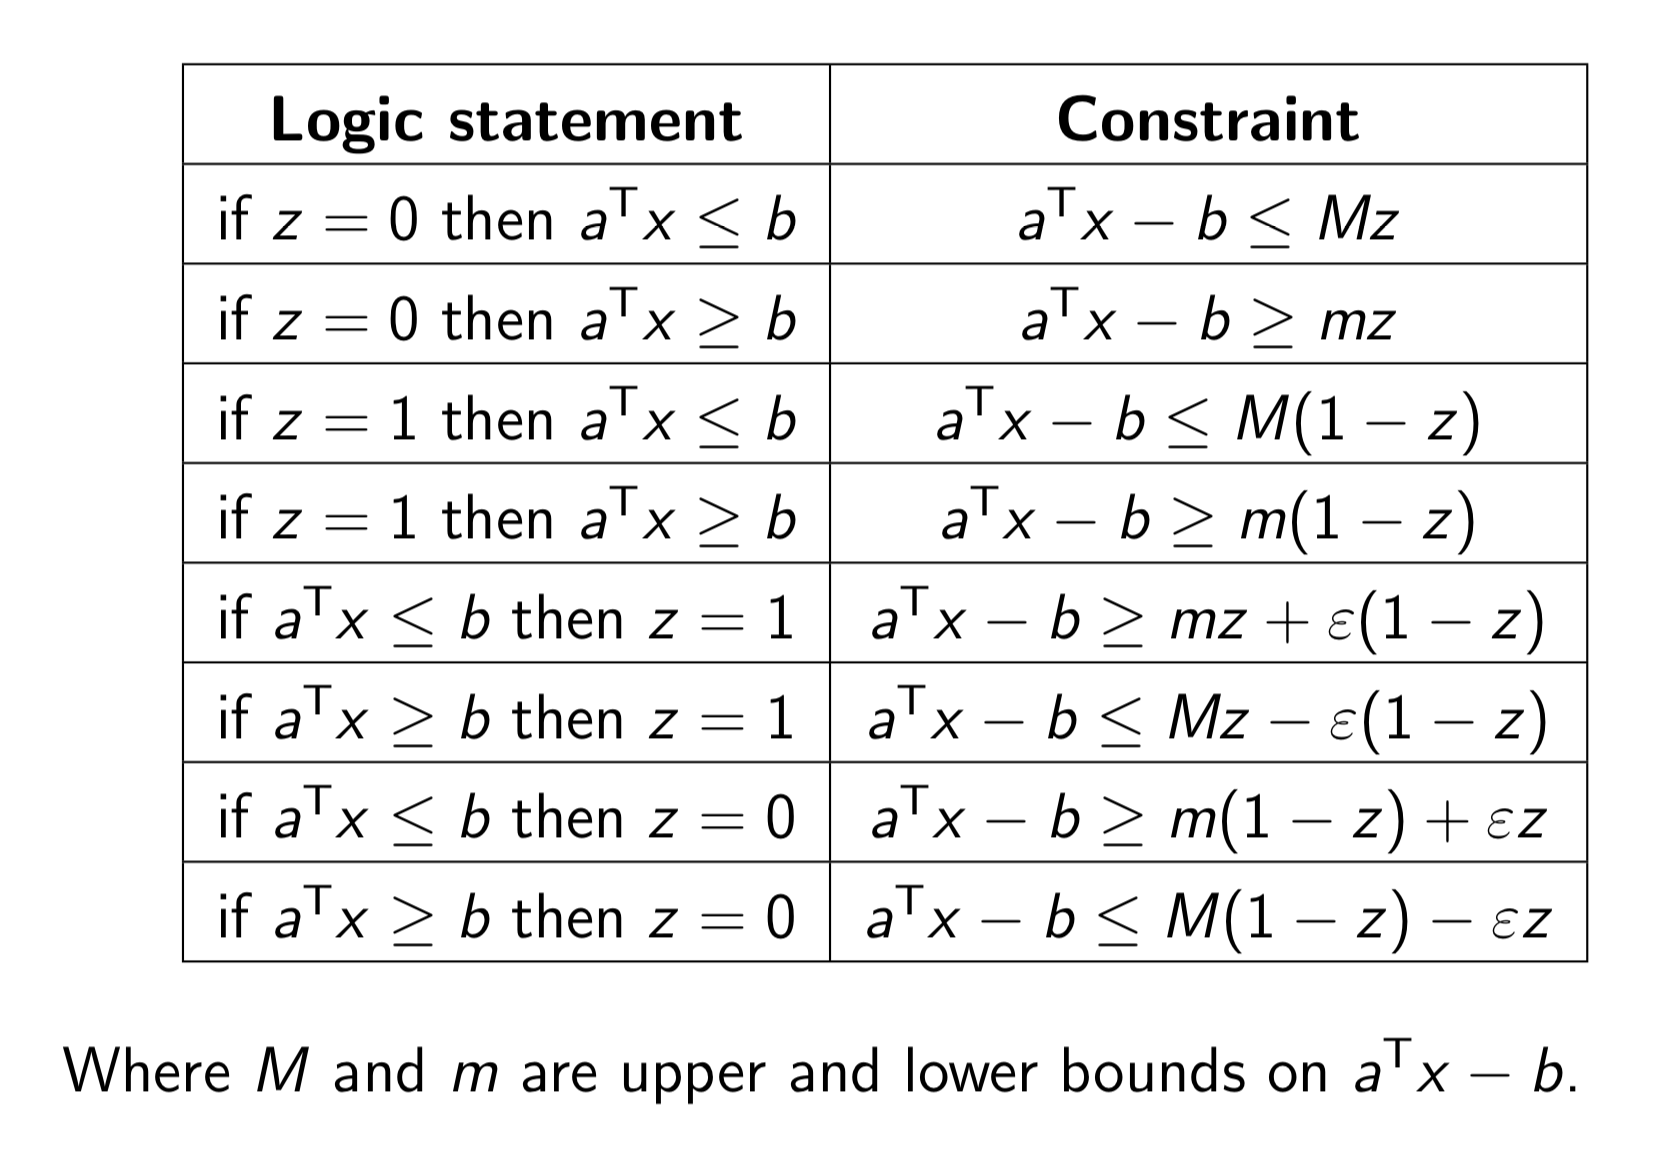
\includegraphics[scale = 0.4]{table-if-then}\footnotemark
\end{center}
\caption{If/then models with a constraint and a binary variable.}
\end{table}
\footnotetext{This table was taken from notes by Laurent Lassard.}

\subsection{Binary reformulation of integer variables}
If an integer variable has small upper and lower bounds, it can sometimes be advantageous to recast it as a sequence of binary variables - for either modeling, the solver, or both.   Although there are technically many ways to do this, here are the two most common ways.

\begin{general}{Full reformulation}{\textcolor{blue}{$u$ many binary variables}}
\label{general:full-reformulation}
For a non-negative integer variable $x$ with upper bound $u$, modeled as 
\begin{equation}
0 \leq x \leq u, \ \ \ \ x \in \Z,
\end{equation}
this can be reformulated with $u$ binary variables $z_1, \dots, z_u$ as 
\begin{equation}
\begin{split}
x & = \sum_{i=1}^u i z_i = z_1 + 2 z_2 + \dots + u z_u\\
1 & \geq \sum_{i=1}^u z_i = z_1 + z_2 + \dots + z_u\\
z_i & \in \{0,1\} \ \ \text{ for } i=1, \dots, u
\end{split}
\end{equation}
\end{general}
We call this the \emph{full reformulation} because there is a binary variable $z_i$ associated with every value $i$ that $x$ could take.  That is, if $z_3 = 1$, then the second constraint forces $z_i = 0$ for all $i \neq 3$ (that is, $z_3$ is the only non-zero binary variable), and hence by the first constraint, $x = 3$.

\begin{general}{Full reformulation}{\textcolor{blue}{$O(\log u)$ many binary variables}}
\label{general:log-reformulation}
For a non-negative integer variable $x$ with upper bound $u$, modeled as 
\begin{equation}
0 \leq x \leq u, \ \ \ \ x \in \Z,
\end{equation}
this can be reformulated with $u$ binary variables $z_1, \dots, z_{\log(\lfloor u \rfloor)+ 1}$ as 
\begin{equation}
\begin{split}
x & = \sum_{i=0}^{\log(\lfloor u \rfloor)+ 1}2^i z_i = z_0 + 2 z_1 +  4 z_2 + 8 z_3 + \dots + 2^{\log(\lfloor u \rfloor) + 1} z_{\log(\lfloor u \rfloor)+ 1}\\
z_i & \in \{0,1\} \ \ \text{ for } i=1, \dots, \log(\lfloor u \rfloor)+ 1
\end{split}
\end{equation}
\end{general}
We call this the \emph{log reformulation} because this requires only logarithmically many binary variables in terms of the upper bound $u$.   This reformulation is particularly better than the full reformulation when the upper bound $u$ is a ``larger" number, although we will leave it ambiguous as to how larger a number need to be in order to be described as a ``larger" number. 
\subsection{SOS1 Constraints}
\begin{definition}
A Special Ordered Sets of type 1 (SOS1) constraint on a vector indicates that \emph{at most one element of the vector can non-zero}.
\end{definition}
We next give an example of how to use binary variables to model this and then show how much simpler it can be coded using the SOS1 constraint.

\begin{examplewithcode}{SOS1 Constraints}{code:SOS1}
\label{example:sos1}
Solve the following optimization problem: \[\begin{aligned}
\text{maximize}\quad & 3x_1 + 4x_2 + x_3 + 5x_4 \\
\text{subject to}\quad & 0 \le x_i \le 5 \\
& \text{at most one of the $x_i$ can be nonzero}
\end{aligned}\]
\end{examplewithcode}
\subsection{SOS2 Constraints}
\begin{definition}
A Special Ordered Sets of type 2 (SOS2) constraint on a vector indicates that \emph{at most two elements of the vector can non-zero AND the non-zero elements must appear consecutively}.
\end{definition}
We next give an example of how to use binary variables to model this and then show how much simpler it can be coded using the SOS2 constraint.
\begin{examplewithcode}{SOS2}{code:SOS2}
\label{example:SOS2}
Solve the following optimization problem: \[\begin{aligned}
\text{maximize}\quad & 3x_1 + 4x_2 + x_3 + 5x_4 \\
\text{subject to}\quad & 0 \le x_i \le 5 \\
& \text{at most two of the $x_i$ can be nonzero} \\
& \text{and the nonzero $x_i$ must be consecutive}
\end{aligned}\]
\end{examplewithcode}

\subsection{Piecewise linear functions with SOS2 constraint}
\begin{examplewithcode}{Piecewise Linear Function}{code:pwl}
\label{example:pwl}
Consider the piecewise linear function 
 $c(x)$ given by
$$
c(x) = 
\begin{cases}
25x  & \text{ if } 0 \leq x \leq 5\\
20x + 25 & \text{ if } 5 \leq x \leq 10\\
15x + 75 & \text{ if } 10 \leq x \leq 15
\end{cases}
$$
\begin{center}
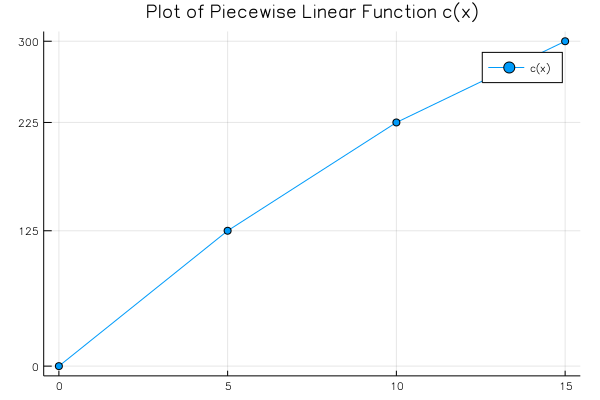
\includegraphics[scale = 0.2]{pwl-plot.png}
\end{center}
We will use integer programming to describe this function.  We will fix $x = a$ and then the integer program will set the value $y$ to $c(a)$.
\begin{align*}
\min\quad & 0\\
\text{Subject to} \quad & x - 5 z_{2} - 10 z_{3} - 15 z_{4} = 0\\
 & y - 125 z_{2} - 225 z_{3} - 300 z_{4} = 0\\
 & z_{1} + z_{2} + z_{3} + z_{4} = 1\\
 & z_{1} - w_{1} \leq 0\\
 & z_{2} - w_{2} \leq 0\\
 & z_{3} - w_{3} \leq 0\\
 & z_{4} - w_{4} \leq 0\\
 & SOS2: \{w_1, w_2, w_3, w_4\}\\
 & 0 \leq z_{i} \leq 1 \quad\forall i \in \{1,2,3,4\}\\
 & w_{i} \in \{0,1\} \quad\forall i \in \{1,2,3,4\}\\
 & x = a\\
\end{align*}

\end{examplewithcode}

\begin{examplewithcode}{Piecewise Linear Function Application}{code:pwl-application}
\label{example:pwl-application}
Consider the following optimization problem where the objective function includes the term $c(x)$, where $c(x)$ is the piecewise linear function described in \nameref{example:pwl}:
$$
\begin{array}{cc}
\max & z = 12x_{11} + 12x_{21} + 14x_{12} + 14x_{22} - c(x)\\
\text{s.t.} & x_{11} + x_{12} \leq x + 5\\
& x_{21} + x_{22} \leq 10\\
& 0.5 x_{11} - 0.5x_{21} \geq 0\\
& 0.4 x_{12} - 0.6 x_{22} \geq 0\\
& x_{ij} \geq 0\\
& 0 \leq x \leq 15
\end{array}
$$

Given the piecewise linear, we can model the whole problem explicitly as a mixed-integer linear program.

 \begin{align*}
 \max\quad & 12 X_{1,1} + 12 X_{2,1} + 14 X_{1,2} + 14 X_{2,2} - y\\
\text{Subject to} \quad & x - 5 z_{2} - 10 z_{3} - 15 z_{4} = 0\\
 & y - 125 z_{2} - 225 z_{3} - 300 z_{4} = 0\\
 & z_{1} + z_{2} + z_{3} + z_{4} = 1\\
 & z_{1} - w_{1} \leq 0\\
 & z_{2} - w_{2} \leq 0\\
 & z_{3} - w_{3} \leq 0\\
 & z_{4} - w_{4} \leq 0\\
 & X_{1,1} + X_{1,2} - x \leq 5\\
 & X_{2,1} + X_{2,2} \leq 10\\
 & 0.5 X_{1,1} - 0.5 X_{2,1} \geq 0\\
 & 0.4 X_{1,2} - 0.6 X_{2,2} \geq 0\\
 & SOS2: \{w_1, w_2, w_3, w_4\}\\
 & X_{i,j} \geq 0 \quad\forall i \in \{1,2\}, j \in \{1,2\}\\
 & 0 \leq z_{i} \leq 1 \quad\forall i \in \{1,2,3,4\}\\
 & w_{i} \in \{0,1\} \quad\forall i \in \{1,2,3,4\}\\
 & 0 \leq x \leq 15\\
 & y\\
\end{align*}

\end{examplewithcode}


\subsection{Maximizing a minimum}
When the constraints could be general, we will write $x \in X$ to define general constraints.  For instance, we could have $X = \{ x \in \R^n : Ax \leq b\}$ of $X  = \{ x \in \R^n : Ax \leq b, x \in \Z^n\}$ or many other possibilities.  


Consider the problem 

\begin{align*}
\max   \quad & \min \{x_1, \dots, x_n\}\\
\text{ such that } \quad &  x \in X
\end{align*}
Having the minimum on the inside is inconvenient.  To remove this, we just define a new variable $y$ and enforce that $y \leq x_i$ and then we maximize $y$.  Since we are maximizing $y$, it will take the value of the smallest $x_i$.  Thus, we can recast the problem as

\begin{align*}
\max\quad    & y\\
\text{ such that } \quad  & y \leq x_i \ \text{ for }\  i=1, \dots, n \\
&  x \in X
\end{align*}


\subsection{Relaxing (nonlinear) equality constraints}

There are a number of scenarios where the constraints can be relaxed without sacrificing optimal solutions to your problem.   In a similar vein of the maximizing a minimum, if because of the objective we know that certain constraints will be tight at optimal solutions, we can relax the equality to an inequality.   For example, 
\begin{align*}
\max   \quad &x_1 + x_2 +  \dots + x_n\\
\text{ such that } \quad &  x_i = y_i^2 + z_i^2 \text{ for } i=1, \dots, n
\end{align*}






\section{Notes from AIMMS modeling book.}
\subsection{Guidelines for Integer Programming Modeling}
Practical guidelines for solving difficult MILPs
\url{http://inside.mines.edu/~anewman/MIP_practice120212.pdf}

\subsection{Linear Programming Modeling}
\url{https://download.aimms.com/aimms/download/manuals/AIMMS3OM_LinearProgrammingTricks.pdf}

\subsection{From AIMMS}
 \url{https://download.aimms.com/aimms/download/manuals/AIMMS3OM_FormulatingOptimizationModels.pdf}

%\includegraphics[scale = 0.7, page = 3, trim= 3cm 0 0 3cm]{sections/AIMMS3OM-IntegerProgrammingTricks.pdf}
%\includegraphics[scale = 0.7, page = 4, trim= 3cm 0 0 3cm]{sections/AIMMS3OM-IntegerProgrammingTricks.pdf}
%\includegraphics[scale = 0.7, page = 5, trim= 3cm 0 0 3cm]{sections/AIMMS3OM-IntegerProgrammingTricks.pdf}
%\includegraphics[scale = 0.7, page = 6, trim= 3cm 0 0 3cm]{sections/AIMMS3OM-IntegerProgrammingTricks.pdf}
%\includegraphics[scale = 0.7, page = 7, trim= 3cm 0 0 3cm]{sections/AIMMS3OM-IntegerProgrammingTricks.pdf}
%\includegraphics[scale = 0.7, page = 8, trim= 3cm 0 0 3cm]{sections/AIMMS3OM-IntegerProgrammingTricks.pdf}
%\includegraphics[scale = 0.7, page = 9, trim= 3cm 0 0 3cm]{sections/AIMMS3OM-IntegerProgrammingTricks.pdf}
%\includegraphics[scale = 0.7, page = 10, trim= 3cm 0 0 3cm]{sections/AIMMS3OM-IntegerProgrammingTricks.pdf}
%\includegraphics[scale = 0.7, page = 11, trim= 3cm 0 0 3cm]{sections/AIMMS3OM-IntegerProgrammingTricks.pdf}
%\includegraphics[scale = 0.7, page = 12, trim= 3cm 0 0 3cm]{sections/AIMMS3OM-IntegerProgrammingTricks.pdf}
%\includegraphics[scale = 0.7, page = 13, trim= 3cm 0 0 3cm]{sections/AIMMS3OM-IntegerProgrammingTricks.pdf}
%\includegraphics[scale = 0.7, page = 14, trim= 3cm 0 0 3cm]{sections/AIMMS3OM-IntegerProgrammingTricks.pdf}
\subsubsection{Linear Programming}
Practical guidelines for solving difficult linear programs
\url{https://pdfs.semanticscholar.org/b01f/ad44c20c372fdda95cbfb980c0d37302de07.pdf}

\subsection{Further Topics}

\subsubsection{Precedence Constraints}
\url{https://or.stackexchange.com/questions/1319/best-model-for-precedence-constraints-within-scheduling-problem}


\end{document}
